\chapter{Analyse des opportunités des technologies libres dans le
domaine de l'édition vidéo et prévisions}

\minitoc \newpage

\paragraph{}

Maintenant que les besoins et que les solutions existantes ont été
analysées on rendra compte de la situation actuelle des technologies
libres et de leurs communautés. Il est aussi important de chercher les
raisons qui expliquent que ces logiciels ne sont pas utilisés par les
professionnels. Puis, nous essayerons d'envisager les solutions possibles
qui permettraient de remédier à cette situation.

\paragraph{}

Dans cette partie, nous analyserons la différence entre les manières
d'envisager la création de logiciel et nous verrons quels sont les
avantages et inconvénients de ces fonctionnements. Par la suite nous
nous concentrerons sur les frameworks existants pour faire une analyse
technique des ces technologies. Par la suite, nous analyserons les
communautés qui portent ces différents projets afin d'arriver à voir
les lacunes et les avantages de chacun des projets.  Pour finir, nous
tirerons les conclusions de cette analyse afin de trouver des solutions
aux défis qu'est la création d'un logiciel libre de montage vidéo.

\newpage

\section {Etat actuel de l'offre de logiciel libre}

Le schéma suivant permet de résumer facilement la situation:

\begin{figure} [h]
  \begin{center}
    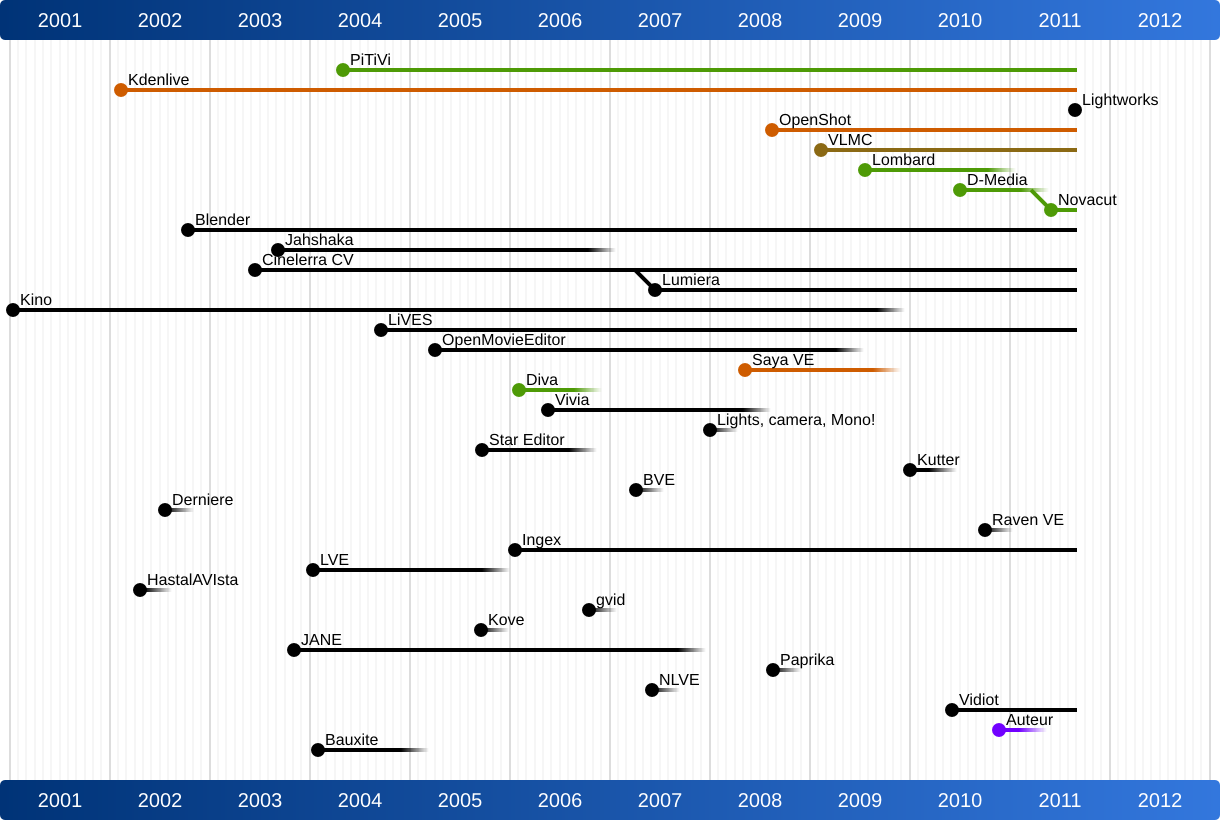
\includegraphics[width=0.9\textwidth]{images/open-source-video-editor-timeline}
  \end{center} \caption{Open source video editors timeline (Auteur:
  Jean-François Fortin, PiTiVi designer)} \label{Yes}
\end{figure}

\paragraph{ }

On constate donc que de nombreux projets de logiciel libre de montage
vidéo on vu le jours ces 10 dernières années, ayant différents
objectifs.  On peu distinguer deux types de publique visés par ces
projets:

\begin {itemize}
  \item {Les amateurs}
  \item {Les professionnels ou semi professionnels}
\end {itemize}

\paragraph {Les amateurs de montages vidéo}

\subparagraph{}

Plusieurs projet, libre permettent ou visent à répondre au besoins
des amateurs, mais à l'heure actuel même ce cas d'utilisation n'est
pas pleinement satisfait par les logiciel libres. Parmi les logiciels
ayant l'objectif de permettre de créer des montage simple on distingue:

\begin {itemize}
  \item {openshot: Logiciel avec de nombreuses fonctionnalité.} \item
  {kino: Logiciel avec peu de fonctionnalité permettant de faire des
    petit montages éfficacement}
  \item {Vidiot qui vise la production de vidéo amateur simple}
\end {itemize}

\paragraph {}

Mais les logiciels ayant pour objectif de pouvoir aux besoins plus
avancés tel que ceux des professionnels (précédemment présenté
dans le cadre de la définition des plus grands acteur du marché)
peuvent être utiliser dans le cadre de montage amateur.

\paragraph{}

Un nouveau projet a aussi récemment vu le jours, ayant un but assez
différent des logiciel actuellement présent. Il s'agit de Novacut,
qui a pour but de permettre aux créateur de film et séries web de
faire le montage de manière collaborative à travers d'Internet, en
partageant les ressources (footage).

\paragraph{}

Cela montre qu'aucun projet n'a encore réussi à s'imposer et ainsi
regrouper les développeurs au sein de projets majeurs. Dans d'autre
domaine, cela a été le cas, par example dans le domaine des lecteurs
vidéo, Vlc a su surpassé ces concurrent, et ainsi supplanté le
marché des lecteur vidéo, qu'il soit libre ou non. Dans le domaine
des environnements de Bureau graphique, KDE et Gnome sont arrivés à un
stade ou leur supériorité technique, et en terme de fonctionnalités
fait d'eux des plateformes de référence.

\paragraph{}

Il est donc intéressant de se demander quel(s) technologie(s),
logiciel(s), pourrai(ent) se voir attribuer cette place dans le monde
de l'édition vidéo libre. Nous allons donc analyser en profondeur,
les logiciel et technologies libre les plus avancés, (précédemment
mentionné dans le cadre de l'analyse de marché: Cinelerra, Kdenlive et
PiTiVi) et ainsi voir si celui-ci, ou ceux-ci, ont le potentiel de pouvoir
un jours rivaliser avec les logiciels propriétaire sur le marché très
fermé du montage vidéo professionnels.

\paragraph{}

Il aurait été intéressant d'analyser le logiciel lightworks, en voit de libération,
mais à l'heure actuel, aucun code n'a été libéré, et par conséquent, celui-ci ne
peut faire partit de cette analyse.

\newpage

\section{Technologies}

\paragraph{}

Pour faire une analyse technique des produits permettant de faire
de l'édition vidéo, il est nécessaire d'analyser le ``core'' des
logiciels, c'est à dire la partie du logiciel où les opérations
d'édition sont effectivement réalisées. Dans ce domaines, il existe
deux façon de procéder:

\begin{itemize} \setlength{\itemsep}{2mm}

  \item{Création d'un logiciel monolithique}

  \item{Création d'un framework \glossary {name={framework, framework},
   description={ Un framework est un ensemble d'outils et de composants
   logiciels organisés conformément à un plan d'architecture et des
   design patterns.}} \index{framework}}

\end{itemize}

\subsection {Technologies monolithique VS technologies modulaires,
frameworks}

\subsubsection{Logiciels monolithiques} %FIXME Look for a def

\paragraph{}

Le conception monolithique dans le cadre des logiciels d'édition vidéo,
consiste au sein d'un même entité de code:

\begin{itemize} \setlength{\itemsep}{2mm}
  \item { la partie graphique et la partie de calculs
    permettant la gestion de tout ce que l'édition non linéaire
    implique}
  \item {L'interface utilisateur.}
\end {itemize}

\paragraph{}

Par le terme logiciel monolithique, il convient de comprendre que le
logiciel peut utiliser des librairies externes, mais le core de ce même
logiciel, et la logique d'édition linéaire à proprement parler est
directement faite à l'intérieur du logiciel et non par une librairie
où framework \index{framework} externe. Cela a pour principal avantage que la conception
est simplifiée pour plusieurs raisons à savoir:

\paragraph{}

Les logiciels professionnels (commerciaux) utilisent très probablement
tous ce mode de fonctionnement (même si probablement, en interne il
ont un core qui ressemble fortement à un framework \index{framework}). Au niveau des
logiciels libres, le logiciel Cinelerra est un exemple dans lequel les
développeurs ont décidé d'utiliser ce mode de fonctionnement.

On peu voir plusieurs conséquences immédiate de ce mode de
développement:

\begin{itemize} \setlength{\itemsep}{2mm}
  \item {Les développeurs n'ont pas la nécessité de penser
    en terme d'interface publique de programmation (API\index{API}), et
    n'ont pas à garantir la stabilité de celle-ci. Cela a pour effet que
    la qualité de l'architecture risque de ne pas être optimale puisque
    la création d'API\index{API} oblige les développeurs/architectes
    à réellement analyser les besoins de manière plus large dès le
    début de la conception. Dans le cas où l'on ne crée pas d'interface
    publique de programmation voué à être réutilisée, le risque est
    que le travail de design et d'architecture ne soit pas réalisé,
    et que le code grandisse de manière anarchique avec les différents
    développeurs qui ajoute leur morceau au fur qu'ils en ont besoin.}
  \item {Les développeurs n'ont besoin de penser l'architecture que pour
    les seuls cas d'utilisation qui sont liés à ce même logiciel,
    ils n'ont pas à voir au delà de ces use cases.}
  \item {Les erreurs en terme de design n'ont pas d'incidences aussi
    graves que dans le cas d'un framework\index{framework}.}
\end {itemize}

\paragraph{}

On se rend compte que cette manière de faire a pour principal avantage
le fait que le logiciel peut être développé plus rapidement puisque
le core du logiciel, et donc le code qui implémente la logique de
l'édition non linéaire est conçue avec pour seul cas d'utilisation,
celui du logiciel. Cependant, de nombreux inconvénients existent de
par la nature monolithique du design:

\subparagraph{Besoins en main d'oeuvre considérables:}

\subparagraph { }

Dans le cadre de logiciel d'édition vidéo, le code à produire
est considérable, comme le montre les statistiques (Annexes 2). Le
logiciel Cinelerra à lui seul fait plus d'un million de lignes. Une
telle quantité de code est difficile à maintenir et requiert des
ressources importantes en terme de main d'oeuvre. Le fait que le logiciel
soit monolithique implique que celui-ci va être utilisé que par ce
logiciel, et par conséquent, les développeurs ne peuvent conté sur
d'autre usage de ce code pour améliorer, développer le core du logiciel.

\paragraph{Réutilisabilité:}

\subparagraph { }

L'un des inconvénients de cette manière de faire est que le code que
l'on a à l'intérieur du logiciel n'est pas réutilisable directement
par d'autres projets, et par conséquent, on peut considérer que cela
est ``individualiste``, chose qu'il convient d'éviter dans le cadre du
développement de logiciel libre afin de ne pas multiplier les efforts,
et dupliquer le code.

\paragraph{}

Cette façon de faire a été utilisée par le projet Cinelerra. Ce
logiciel est le plus avancé en terme de fonctionnalités que le marché
des logiciels libres de montage offre. On peut penser que son architecture
monolithique expliquer ce développement plus abouti. Bien qu'il y ait
évidemment de nombreux autre facteurs tel que le fait que ce logiciel
a été développé par la société Heroine Virtual.

\subsubsection {Les frameworks \index{framework}}

L'autre possibilité est de séparer en deux parties logiciel bien distincts
l'implémentation de la logique de l'édition, lecture, encoding vidéo, de la
partie graphique, interaction avec l'utilisateur final.

L'ensemble forme un
squelette de programme., et ensuite de créer une interface graphique
utilisant ce cadre logiciel. La plupart des logiciels libres ont suivi ce
plan de conception. Le logiciel PiTiVi utilise le Framework multimedia
GStreamer alors que KDEnlive utilise le framework\index{framework} orienté édition et
broadcasting MLT. Dans le cadre des Frameworks, nous nous intéresserons
en particulier à l'analyse de ceux-ci puisque les notions relatives
à l'édition vidéo, et la gestion de toute la partie multimédia est
réalisée par ceux-ci. Les logiciels d'édition ne sont à priori que
de simples interfaces graphiques basées sur ces frameworks, et par
conséquent leur analyse ne présente qu'un faible intérêt.


\section{Analyse technique}

\section{Analyse des communauté}

\section{Lacunes}

\section{Solutions possibles}
